% ============================================================================
%  ACADEMIC REPORT — DOOM AUV Simulation (English Version)
%  Compile with: pdflatex Memoria_DOOM_AUV_EN.tex  (x2 for references)
% ============================================================================
\documentclass[10pt,twocolumn,letterpaper]{article}

% ----- Packages -----
\usepackage[utf8]{inputenc}
\usepackage[T1]{fontenc}
\usepackage[english]{babel}
\usepackage{times}
\usepackage{graphicx}
\usepackage{amsmath,amssymb}
\usepackage{hyperref}
\usepackage{url}
\usepackage{booktabs}
\usepackage{multirow}
\usepackage{xcolor}
\usepackage{listings}
\usepackage{float}
\usepackage{caption}
\usepackage{subcaption}
\usepackage{geometry}
\usepackage{titlesec}
\usepackage{enumitem}
\usepackage{fancyhdr}
\usepackage{abstract}

\geometry{letterpaper, left=1.8cm, right=1.8cm, top=2.2cm, bottom=2.2cm}

% ----- Listings configuration -----
\definecolor{codebg}{rgb}{0.95,0.95,0.97}
\definecolor{codegreen}{rgb}{0.0,0.5,0.0}
\definecolor{codegray}{rgb}{0.5,0.5,0.5}
\definecolor{codepurple}{rgb}{0.58,0,0.82}

\lstdefinestyle{pythonstyle}{
    backgroundcolor=\color{codebg},
    commentstyle=\color{codegreen},
    keywordstyle=\color{blue}\bfseries,
    numberstyle=\tiny\color{codegray},
    stringstyle=\color{codepurple},
    basicstyle=\ttfamily\scriptsize,
    breakatwhitespace=false,
    breaklines=true,
    captionpos=b,
    keepspaces=true,
    numbers=left,
    numbersep=4pt,
    showspaces=false,
    showstringspaces=false,
    showtabs=false,
    tabsize=2,
    frame=single,
    rulecolor=\color{codegray},
    language=Python
}
\lstset{style=pythonstyle}

% ----- Section formatting -----
\titleformat{\section}{\large\bfseries}{\thesection.}{0.5em}{}
\titleformat{\subsection}{\normalsize\bfseries}{\thesubsection}{0.5em}{}
\titleformat{\subsubsection}{\small\bfseries\itshape}{\thesubsubsection}{0.5em}{}

% ----- Metadata -----
\hypersetup{
    colorlinks=true,
    linkcolor=blue!70!black,
    citecolor=blue!70!black,
    urlcolor=blue!70!black,
    pdftitle={AUV Simulation with ROS 2 Architecture and DOOM-Style Rendering Engine},
    pdfauthor={Sergio}
}

% ============================================================================
\begin{document}

% ----- Title -----
\twocolumn[
\begin{@twocolumnfalse}
\begin{center}
    {\LARGE\bfseries Simulation of an Autonomous Underwater Vehicle \\
    with a Distributed ROS\,2 Architecture and \\
    \textit{DOOM}-Style First-Person Rendering Engine\par}
    \vspace{0.8em}
    {\large Sergio --- al428707@uji.es\par}
    \vspace{0.3em}
    {\normalsize Universitat Jaume I --- Engineering Degree\\
    Course: Aerial and Underwater Systems\par}
    \vspace{0.3em}
    {\normalsize February 2026\par}
    \vspace{1.2em}
\end{center}

% ----- Abstract -----
\begin{onecolabstract}
\noindent
This work describes the design, implementation, and validation of \textbf{DOOM AUV Sim}, a comprehensive Autonomous Underwater Vehicle (AUV) simulator built on the ROS\,2 Humble middleware and the Python programming language. The system integrates a first-person rendering engine based on 2.5D raycasting ---inspired by the classic video game \textit{DOOM} (1993)---, an underwater physics engine with hydrodynamic inertia and battery consumption, an acoustic underwater communication channel with latency and packet loss modeled according to Thorp's absorption formula, and an onboard autonomy module featuring a control architecture inspired by Brooks' subsumption paradigm. The distributed architecture employs six ROS\,2 nodes interconnected through approximately twenty Pub/Sub topics, without resorting to Services or Actions, a design choice justified by the inherently asynchronous and variable-latency nature of the underwater domain. The system was developed iteratively over multiple design-implementation-test cycles, progressively resolving issues related to depth control stability, robotic arm alignment, realistic acoustic communication, and target capture. The results demonstrate that the simulator enables the autonomous collection of five randomly distributed targets, the reactive avoidance of both dynamic and static obstacles, and the export of the explored map in PCD, PNG, and OBJ formats.
\end{onecolabstract}
\vspace{1em}
\end{@twocolumnfalse}
]

% ============================================================================
\section{Introduction}
\label{sec:introduction}

Autonomous Underwater Vehicles (AUVs) represent one of the most challenging robotic platforms in engineering. Unlike terrestrial or aerial robots, AUVs operate in an environment where conventional electromagnetic communication ---including GPS--- becomes infeasible beyond a few meters of depth. The standard alternative, acoustic underwater communication, introduces latencies on the order of hundreds of milliseconds to seconds and significant packet loss rates, severely limiting real-time teleoperation capability~\cite{stojanovic2009}.

In this context, the development of simulators that faithfully reproduce these operational constraints constitutes a critical need both for operator training and for the validation of autonomy algorithms. However, most existing AUV simulators ---such as UUV Simulator~\cite{uuvsim2016} or Stonefish~\cite{stonefish2020}--- focus on the physical fidelity of the underwater medium or on integration with planning frameworks like Nav2, but do not necessarily expose the robot's perceptual and communication limitations to the user in an intuitive manner.

This project proposes an alternative approach: an AUV simulator that uses a first-person rendering engine inspired by the classic DOOM (id Software, 1993) to immersively represent the limited perspective of the vehicle's forward-looking sonar. This 2.5D raycasting, combined with a fog-of-war system, forces the operator to experience the same sensory constraints as the actual AUV, facilitating an intuitive understanding of its capabilities and limitations.

The system was built entirely on ROS\,2 Humble, leveraging its Pub/Sub communication model to implement a distributed architecture of six nodes that clearly separates the responsibilities of simulation, communication, arbitration, autonomy, and visualization. Throughout its iterative development, multiple technical challenges related to control stability, acoustic channel fidelity, and robotic arm coordination were addressed and resolved.

% ============================================================================
\section{Related Work}
\label{sec:related_work}

\subsection{AUV Simulation in ROS\,2}

The ROS\,2 ecosystem offers several options for underwater vehicle simulation. The UUV Simulator package~\cite{uuvsim2016}, originally developed for ROS\,1, provides detailed hydrodynamic models in Gazebo, but its configuration complexity and the computational requirements of full three-dimensional physics simulation make it poorly suited for rapid iteration. Stonefish~\cite{stonefish2020} offers a lighter-weight simulator with native ROS\,2 support, but still requires URDF models, world files, and complex sensor configuration.

These simulators prioritize physical fidelity over accessibility and rapid prototyping. In contrast, the approach adopted in this work prioritizes \textbf{functional fidelity}: the operational effects (latency, packet loss, limited field of view, inertia) are replicated without the need for a full three-dimensional physics simulation.

\subsection{Underwater Acoustic Communication}

Sound propagation underwater is governed by frequency-dependent absorption, geometric spreading, and variable channel effects. Thorp's formula~\cite{thorp1967} provides a practical approximation to the absorption coefficient $\alpha$ in dB/km for a frequency $f$ in kHz:

\begin{equation}
\alpha = \frac{0.11 f^2}{1 + f^2} + \frac{44 f^2}{4100 + f^2} + 2.75 \times 10^{-4} f^2 + 0.003
\label{eq:thorp}
\end{equation}

The Transmission Loss (TL) combines geometric spreading and absorption:

\begin{equation}
TL = 20 \log_{10}(R) + \alpha \cdot R \cdot 10^{-3} \quad [\text{dB}]
\label{eq:tl}
\end{equation}

where $R$ is the distance in meters. The resulting Signal-to-Noise Ratio (SNR) is computed as $\text{SNR} = SL - TL - NL$, where $SL$ is the source level and $NL$ is the ambient noise level~\cite{urick1983}.

\subsection{Subsumption Architecture}

The subsumption architecture, proposed by Brooks~\cite{brooks1986}, organizes robotic control into behavioral layers with strict priority. Lower layers (reactive survival behaviors) can \textit{suppress} the outputs of higher layers (goal-oriented behaviors). This paradigm is particularly well-suited for dynamic and unpredictable environments such as the ocean floor, where obstacle avoidance must take absolute priority over any mission objective.

% ============================================================================
\section{Hypothesis and Design}
\label{sec:hypothesis}

The central hypothesis of this work is that a \textbf{lightweight AUV simulator based exclusively on ROS\,2 Pub/Sub communication and 2.5D rendering} can reproduce the essential operational constraints of a real underwater vehicle ---acoustic latency, limited perception, hydrodynamic inertia--- with sufficient functional fidelity to validate autonomy algorithms and train operators, without requiring the complexity of a full three-dimensional physics simulator.

The design is founded on three premises:

\begin{enumerate}[leftmargin=*,itemsep=2pt]
    \item \textbf{Strict simulation-control separation:} The simulation engine publishes ground truth on isolated topics (\texttt{/sim/*}), and a bridge node introduces delay before republishing them as AUV perception (\texttt{/auv/*}).
    \item \textbf{Realistic communication as a requirement, not an option:} All operator commands must traverse the simulated acoustic channel. No direct communication shortcuts exist.
    \item \textbf{Safety through subsumption:} Obstacle avoidance and battery failsafe behaviors can override both autonomous and manual control.
\end{enumerate}

% ============================================================================
\section{Methodology}
\label{sec:methodology}

\subsection{Overall System Architecture}

The system consists of six custom ROS\,2 nodes, an external visualization node (RViz\,2), and a teleoperation node executed in a separate terminal. Figure~\ref{fig:topology} presents the complete topology.

\begin{figure}[H]
    \centering
    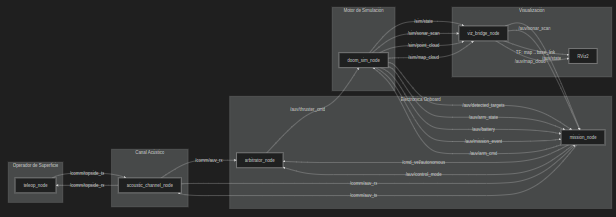
\includegraphics[width=\linewidth]{rqt_graph.png}
    \caption{ROS\,2 system topology (\texttt{rqt\_graph}). Nodes are grouped into five functional domains: Topside, Acoustic Channel, Onboard, Simulator, and Visualization.}
    \label{fig:topology}
\end{figure}

Table~\ref{tab:nodes} summarizes the nodes and their responsibilities.

\begin{table}[H]
\centering
\caption{ROS\,2 system nodes and their roles.}
\label{tab:nodes}
\scriptsize
\begin{tabular}{@{}lp{5.2cm}@{}}
\toprule
\textbf{Node} & \textbf{Responsibility} \\
\midrule
\texttt{doom\_sim\_node} & Simulation engine: physics, Pygame rendering, sensor publishing \\
\texttt{teleop\_node} & Terminal-based operator interface with dashboard \\
\texttt{acoustic\_channel\_node} & Bidirectional channel with latency and packet loss \\
\texttt{arbitrator\_node} & Manual/Auto command multiplexer \\
\texttt{mission\_node} & Onboard autonomy logic with finite state machine \\
\texttt{viz\_bridge\_node} & Delayed bridge for RViz\,2 (TF + PointCloud) \\
\bottomrule
\end{tabular}
\end{table}

The decision to use exclusively Pub/Sub topics ---without ROS\,2 Services or Actions--- stems from the fundamentally asynchronous nature of the domain. A ROS\,2 Service is blocking: the client waits for the server response. In a scenario where communication may take seconds or be lost entirely, this pattern would cause unacceptable deadlocks in the control loop. Actions, although asynchronous with feedback support, would introduce state management complexity that is more directly resolved through the mission node's state machine combined with topic-based events.

\subsection{Simulation Engine}

The \texttt{doom\_sim\_node} runs a main loop at 20\,Hz that integrates three subsystems: the underwater physics, the rendering engine, and the ROS\,2 interface.

\subsubsection{Physics Engine}

The physics engine models an AUV with three controllable degrees of freedom: linear advance, yaw rotation, and vertical movement. Rather than directly assigning velocity from received commands, the system applies a model of \textbf{cumulative hydrodynamic inertia}. Commands from \texttt{/auv/thruster\_cmd} (type \texttt{Twist}) are interpreted as forces that accelerate the vehicle:

\begin{lstlisting}[caption={Acceleration and hydrodynamic drag model.}, label={lst:physics}]
# Acceleration: commands accumulate velocity
self.linear_vel += cmd.linear.x * FORCE_LINEAR
self.angular_vel += cmd.angular.z * FORCE_ANGULAR
self.z_vel += cmd.linear.z * FORCE_Z

# Hydrodynamic drag: per-tick decay
self.linear_vel *= WATER_DRAG_LINEAR   # 0.92
self.angular_vel *= WATER_DRAG_ANGULAR # 0.85
self.z_vel *= WATER_DRAG_LINEAR
\end{lstlisting}

The drag factor $d = 0.92$ implies that, in the absence of external forces, velocity decays exponentially as $v(t) = v_0 \cdot d^t$, producing smooth motion with perceptible inertia. Collision is resolved through direct cell-map checking and obstacle proximity verification, including logic that allows the vehicle to escape if it is already within the collision radius.

The battery model implements heterogeneous consumption: a base drain of $0.001$ units per tick plus contributions proportional to linear velocity ($|\dot{x}| \times 0.005$), angular velocity ($|\dot{\theta}| \times 0.01$), and vertical velocity ($|\dot{z}| \times 0.01$).

\subsubsection{Rendering Engine}

The rendering employs the raycasting technique~\cite{lodev_raycasting}, where 120 rays are cast from the AUV's position across a $60^{\circ}$ arc (\texttt{FOV = $\pi/3$}). For each ray, the algorithm advances iteratively in 5-pixel increments until a wall is detected or the maximum depth (100 units) is reached. The perpendicular distance is computed by applying fisheye correction:

\begin{equation}
d_{\perp} = d_{\text{raw}} \cdot \cos(\theta_{\text{player}} - \theta_{\text{ray}})
\label{eq:fisheye}
\end{equation}

The rendered column height is inversely proportional to distance: $h = 21000 / (d_{\perp} + \epsilon)$. Dynamic obstacles (vessels, marine creatures) and static obstacles (reefs, mines) are rendered as billboard sprites with type-differentiated shapes. Collection targets are drawn as circles with an orientation indicator (red line).

A side effect of raycasting is the progressive map revelation (fog of war): each cell traversed by a ray is marked as explored in a boolean matrix \texttt{fog\_map[100$\times$100]}, which controls visibility in both the sonar minimap and the export data.

\begin{figure}[H]
    \centering
    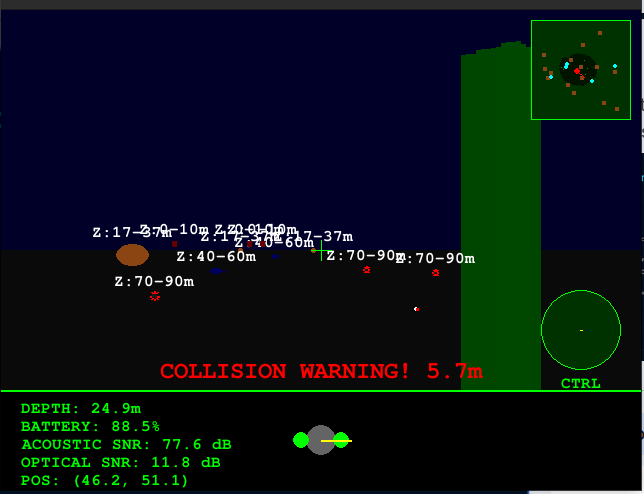
\includegraphics[width=\linewidth]{sim_screenshot.png}
    \caption{DOOM AUV simulator interface. The main view shows the 2.5D raycasting rendering. The bottom HUD displays depth, battery, and SNR. The upper-right minimap shows sonar coverage with fog of war. The robotic arm with gripper is visible at the bottom center.}
    \label{fig:interface}
\end{figure}

\subsection{Acoustic Communication Channel}

The \texttt{acoustic\_channel\_node} implements a bidirectional channel between the surface operator (topside) and the AUV's onboard electronics. Each JSON message entering through \texttt{/comm/topside\_tx} (downlink) or \texttt{/comm/auv\_tx} (uplink) is enqueued with a delay computed as:

\begin{equation}
\tau = \frac{R}{c_s} + U(0.01, 0.05) \quad [\text{s}]
\label{eq:delay}
\end{equation}

where $R$ is the distance to the AUV, $c_s = 1500$\,m/s is the speed of sound in water, and $U(a,b)$ is a uniform random component modeling processing jitter. Additionally, each packet has a 5\% probability of loss, independently and identically distributed.

The \texttt{CommunicationPhysics} module implements the complete acoustic SNR model according to Equation~\ref{eq:tl} with Thorp absorption (Equation~\ref{eq:thorp}) at $f = 25$\,kHz and $SL = 185$\,dB re 1\,$\mu$Pa. The optical SNR is modeled with an exponential attenuation ($c = 0.08$\,m$^{-1}$, range 100\,m) corresponding to clear oceanic water. A simplified scintillation model introduces random 5\% signal drops simulating the effect of internal waves.

\subsection{Control Architecture}

\subsubsection{Command Arbitration}

The \texttt{arbitrator\_node} operates as a temporal multiplexer: at each tick of its 20\,Hz loop, it publishes to \texttt{/auv/thruster\_cmd} the most recent command received from the active source (manual or autonomous), provided that command is recent ($< 0.5$\,s). If no recent commands are available, it publishes a null \texttt{Twist}, which the hydrodynamic drag translates into progressive deceleration.

\subsubsection{Safety Subsumption}

The \texttt{mission\_node} implements a priority hierarchy inspired by the subsumption architecture~\cite{brooks1986}. The safety layers operate \textbf{in all modes}, including manual, and can force a switch to autonomous mode:

\begin{enumerate}[leftmargin=*,itemsep=2pt]
    \item \textbf{EMERGENCY\_REVERSE} ($d < 1.5$\,m): Pure reverse for 2\,s. Highest priority.
    \item \textbf{AVOID\_CRITICAL} ($d < 3.0$\,m): Reverse with rotation toward the side with more free space, for 3\,s.
    \item \textbf{BATTERY\_FAILSAFE} (battery $< 10\%$): Forces emergency ascent.
    \item \textbf{Mission states} (EXPLORE, APPROACH, ALIGN, etc.): Active only in AUTO mode.
\end{enumerate}

The evasion direction is determined in real time by comparing the sum of sonar ranges in the left and right hemifields:

\begin{lstlisting}[caption={Evasion direction determination.}, label={lst:evasion}]
mid = len(scan.ranges) // 2
left_sum  = sum(scan.ranges[mid:])
right_sum = sum(scan.ranges[:mid])
turn_dir = 1.0 if left_sum > right_sum else -1.0
\end{lstlisting}

\subsection{Autonomous Mission}

The onboard autonomy is structured as a finite state machine with six main states (Figure~\ref{fig:fsm}).

\begin{figure}[H]
    \centering
    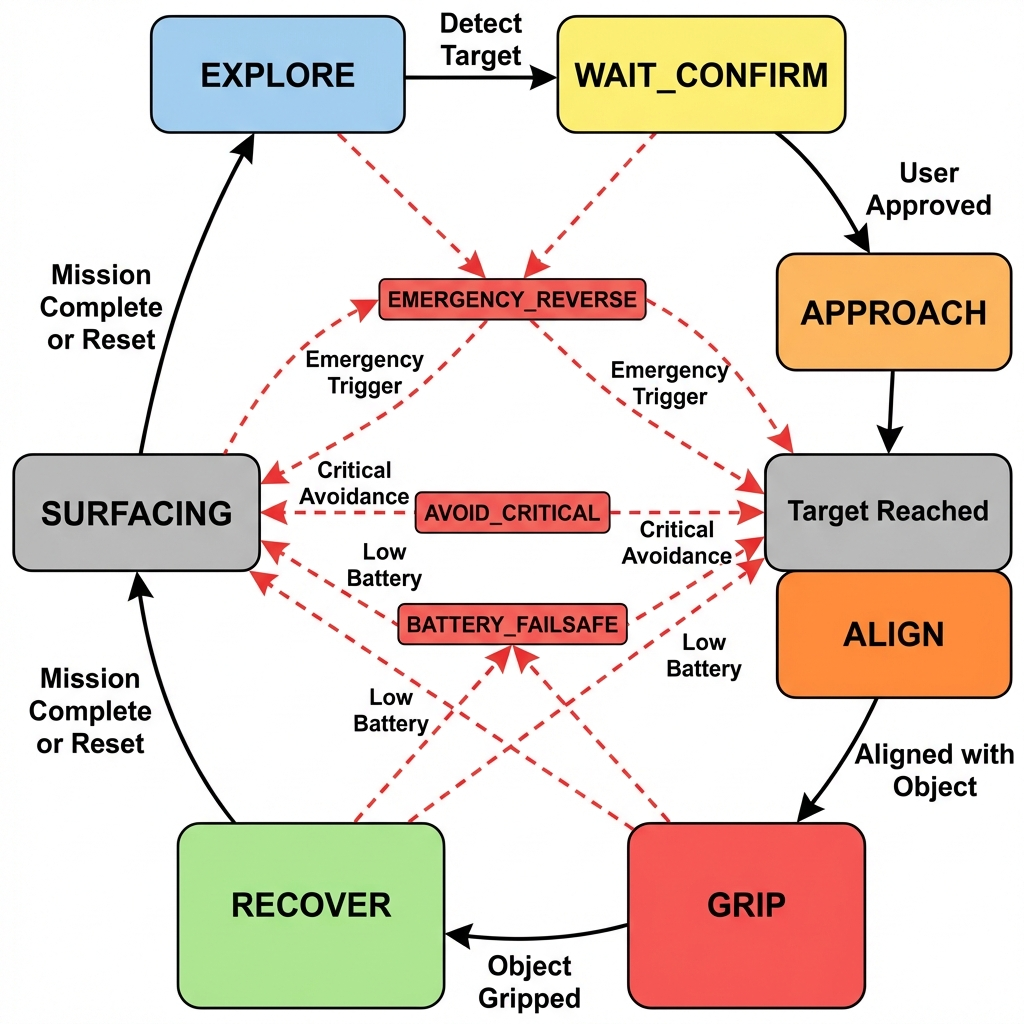
\includegraphics[width=\linewidth]{fsm_diagram.png}
    \caption{Autonomous mission finite state machine. Safety transitions (red lines) can interrupt any state.}
    \label{fig:fsm}
\end{figure}

\textbf{EXPLORE:} The AUV follows a lawnmower pattern (systematic zigzag sweep) defined by a list of waypoints on a grid with 20-unit spacing. Navigation employs a proportional yaw controller with gain $K_p = 0.5$, saturated at $\pm 1.0$\,rad/s. Linear velocity is reduced to $0.2$ when the angular error is large ($|\psi_e| > 0.5$\,rad) to prevent advance during sharp turns.

\textbf{WAIT\_CONFIRM:} When the simulator publishes a visible target on \texttt{/auv/detected\_targets}, the \textit{mission\_node} transitions to a confirmation wait state, publishing updated telemetry. The operator must send a confirmation (\texttt{confirm}) or rejection (\texttt{reject}) through the acoustic channel. Rejected targets are stored to prevent re-detection.

\subsubsection{Approach Controller (APPROACH)}

The APPROACH state implements a \textbf{dual proportional controller} that simultaneously governs the AUV's linear and angular velocities, with the objective of converging on the target by minimizing the Euclidean distance $d = \sqrt{\Delta x^2 + \Delta y^2}$ and the heading error $\psi_e$.

The heading error is computed as the difference normalized to the interval $(-\pi, \pi]$:

\begin{equation}
\psi_e = \left(\text{atan2}(\Delta y, \Delta x) - \psi_{\text{auv}} + \pi\right) \bmod 2\pi - \pi
\label{eq:heading_error}
\end{equation}

where $\psi_{\text{auv}} = 2 \cdot \text{atan2}(q_z, q_w)$ is extracted from the orientation quaternion. The angular control law applies:

\begin{equation}
\omega = \text{clamp}\left(\psi_e \cdot K_\omega,\; -\omega_{\max},\; \omega_{\max}\right)
\label{eq:approach_angular}
\end{equation}

with $K_\omega = 0.3$ and $\omega_{\max} = 0.5$\,rad/s. This gain was reduced from the original value of $0.5$ to prevent aggressive turns that caused overshoot and oscillations around the target.

The linear velocity implements a \textbf{switching scheme with angular dead zone}:

\begin{equation}
v = \begin{cases}
0 & \text{if } |\psi_e| > 0.2 \text{ rad} \\
\text{clamp}\left(0.3 \cdot d,\; 0.1,\; 0.5\right) & \text{otherwise}
\end{cases}
\label{eq:approach_linear}
\end{equation}

The switching at $|\psi_e| = 0.2$\,rad is critical: \textbf{the AUV does not advance unless it is pointing at the target}. This prevents lateral drift which, given non-zero inertia, would accumulate velocity perpendicular to the desired heading. The distance-proportional velocity ($0.3 \cdot d$) provides natural deceleration in the final phase, preventing overshoot.

The transition to ALIGN is triggered when three conditions are jointly satisfied: $d < 1.5$\,m, $|\Delta z| < 2.0$\,m (depth), and $|\psi_e| < 0.3$\,rad. An emergency brake ($v = 0$) is applied unconditionally at $d < 0.5$\,m to prevent collision with the target.

\subsubsection{Alignment and Visual Servoing (ALIGN)}

The ALIGN state constitutes the most complex control module in the system. Unlike APPROACH, which operates in the world's Cartesian space, ALIGN employs \textbf{Image-Based Visual Servoing} (IBVS): the error is defined directly in the screen coordinates $(u, v)$ of the rendered target, and the control action is applied to the robotic arm actuators.

\textbf{Body freeze.} Upon entering ALIGN, the AUV completely halts all body motion ($v = 0$, $\omega = 0$). This design decision avoids an undesirable feedback loop: any body rotation displaces the target image on screen, which would trigger arm corrections, which in turn would alter the relative position. Keeping the body static decouples the two control systems.

\textbf{Arm control.} The arm is controlled through discrete commands (``left'', ``right'', ``up'', ``down'', ``rot\_left'', ``rot\_right'') published at 10\,Hz. To determine which command to issue, the algorithm implements a \textbf{priority policy with interleaving}:

\begin{lstlisting}[caption={ALIGN state visual servoing loop.}, label={lst:align}]
# 1. Rotation - HIGH priority
if abs(diff_deg) >= 5.0:
    if abs(diff_deg) >= 15.0 or tick_even:
        cmd = "rot_right" if diff_deg > 0
              else "rot_left"
# 2. Screen X position
elif abs(cur_x - target_x) > 5:  # px
    cmd = "right" if cur_x < target_x
          else "left"
# 3. Screen Y position
elif abs(cur_y - target_y) > 5:  # px
    cmd = "down" if cur_y < target_y
          else "up"
else:
    pos_aligned = True
\end{lstlisting}

Gripper rotation is computed as the normalized angular difference between the target's absolute orientation (extracted from its quaternion) and the gripper's current angle:

\begin{equation}
\Delta\theta = \left(\theta_{\text{target}} - \theta_{\text{gripper}} + 180^{\circ}\right) \bmod 360^{\circ} - 180^{\circ}
\label{eq:gripper_rotation}
\end{equation}

The interleaving policy (\texttt{tick\_even}) ensures that when the rotation is ``close enough'' ($|\Delta\theta| < 15^{\circ}$) but not ``perfect'' ($|\Delta\theta| \geq 5^{\circ}$), the system alternates between rotation and position corrections on even and odd ticks. This prevents the arm from becoming locked in a purely rotational correction cycle.

\textbf{Creep forward.} Only when both arm position and rotation are aligned but the 3D distance to the target exceeds $1.2$\,m does the system apply a minimal linear advance of $v = 0.1$, bringing the body closer to the object without losing alignment. This logic functions as a proximity bang-bang controller.

Table~\ref{tab:control_params} summarizes the control parameters for both states.

\begin{table}[H]
\centering
\caption{APPROACH and ALIGN controller parameters.}
\label{tab:control_params}
\scriptsize
\begin{tabular}{@{}llcc@{}}
\toprule
\textbf{State} & \textbf{Parameter} & \textbf{Value} & \textbf{Unit} \\
\midrule
APPROACH & $K_\omega$ (heading) & 0.3 & -- \\
APPROACH & $\omega_{\max}$ & 0.5 & rad/s \\
APPROACH & $v$ range & [0.1, 0.5] & m/s \\
APPROACH & Angular dead zone & 0.2 & rad \\
APPROACH & Transition dist. & 1.5 & m \\
\midrule
ALIGN & Rotation tol.\ (strict) & 5.0 & $^{\circ}$ \\
ALIGN & Rotation tol.\ (interleave) & 15.0 & $^{\circ}$ \\
ALIGN & Screen position tol. & 5 & px \\
ALIGN & Creep $v$ & 0.1 & m/s \\
ALIGN & Grip dist.\ ($d_{3D}$) & 1.2 & m \\
\bottomrule
\end{tabular}
\end{table}

\subsubsection{Grip Verification and Closure (GRIP)}

The ALIGN-to-GRIP transition is triggered when three conditions are simultaneously true: $|\Delta\theta| < 5^{\circ}$, screen-centered position ($|u_e| < 5$\,px and $|v_e| < 5$\,px), and $d_{3D} < 1.2$\,m. After the transition, the rendering module independently verifies three conditions: 3D distance $< 1.5$\,m, gripper angular error $< 30^{\circ}$, and on-screen distance $< 50$\,px. If capture fails, the system returns to ALIGN step 0 and reopens the gripper for a retry.

\subsection{Procedural Environment}

The \texttt{MapManager} generates a procedural underwater world on a $100 \times 100$ cell map. Table~\ref{tab:obstacles} details the obstacle distribution.

\begin{table}[H]
\centering
\caption{Obstacle and target distribution.}
\label{tab:obstacles}
\scriptsize
\begin{tabular}{@{}lcccl@{}}
\toprule
\textbf{Type} & \textbf{N} & \textbf{Depth (m)} & \textbf{Dynamic} & \textbf{Color ID} \\
\midrule
Vessels & 10 & 0--10 & Yes & Red (3) \\
Creatures & 10 & 40--60 & Yes & Blue (4) \\
Reefs & 15 & 17--37 & No & Brown (5) \\
Mines & 15 & 70--90 & No & Gray (6) \\
Targets & 5 & 5--95 & No & Cyan \\
\bottomrule
\end{tabular}
\end{table}

% ============================================================================
\section{Iterative Development Process}
\label{sec:development}

The system was developed through a continuous iterative refinement process spanning over fifteen development cycles. The following sections document the main milestones and technical blockers resolved, organized chronologically.

\subsection{Phase 1: Base Architecture}

The first iteration established the fundamental components: the simulation node with raycasting rendering, the \textit{teleop\_node} with direct communication via \texttt{Twist} topics, and a static map with fixed walls. In this phase, manual control published directly to the \texttt{/cmd\_vel} topic without an intermediate acoustic channel. The physics assigned velocity instantaneously, without inertia.

\subsection{Phase 2: Acoustic Communication and Dashboard}

The \texttt{acoustic\_channel\_node} was introduced as a mandatory intermediary for all operator-AUV communication. The \textit{teleop\_node} was redesigned to package commands as JSON and transmit them via \texttt{/comm/topside\_tx}. The terminal dashboard was implemented using ANSI codes to display real-time telemetry.

A significant blocker was the detection of \textbf{acoustic link disconnection}: the dashboard displayed ``DISCONNECTED'' intermittently because the last-packet timestamp verification was not updating correctly. The solution consisted of updating \texttt{last\_packet\_time} upon reception of \textit{any} valid JSON, regardless of its content.

\subsection{Phase 3: Autonomy and Obstacle Avoidance}

The implementation of the \texttt{mission\_node} with the state machine and subsumption architecture required multiple iterations. The first critical issue was that the \textbf{autopilot did not assume control} when needed: the safety layers failed to force AUTO mode in emergency situations. The solution was to add explicit publishing to \texttt{/auv/control\_mode} from the safety layers.

\subsection{Phase 4: Arm Control and Stabilization}

The robotic arm alignment phase for target capture proved to be the most problematic and required at least six refinement cycles:

\begin{itemize}[leftmargin=*,itemsep=2pt]
    \item \textbf{Misaligned gripper:} The gripper consistently positioned itself to the left of the target. The visual servoing logic was refined to balance rotation and positional adjustment.
    \item \textbf{Capture distance:} Initially set at 3\,m, it proved excessive. It was iteratively reduced to 1.5\,m (verification in \texttt{renderer.py}) and 1.2\,m (transition in \texttt{mission\_node}).
    \item \textbf{Vertical oscillation:} The depth controller with gain $K_p = 1.0$ caused vertical oscillations that prevented capture. The gain was reduced to $K_p = 0.3$ for smoother control.
    \item \textbf{Arm speed:} Rotation and translation speeds of the arm were adjusted to allow precise control without overshoot.
    \item \textbf{Non-closing gripper:} The angular tolerance was relaxed from $5^{\circ}$ to $30^{\circ}$ to allow capture with approximate alignments, which is more operationally realistic.
\end{itemize}

\subsection{Phase 5: Acoustic Realism and 3D Export}

In the final phase, residual direct communication channels were eliminated, ensuring that 100\% of manual control passed through the acoustic channel with latency and packet loss. Map export in Wavefront OBJ format as a 3D mesh was implemented, complementing the existing PCD and PNG formats.

% ============================================================================
\section{Testing and Results}
\label{sec:results}

\subsection{Test Protocol}

Tests were conducted on an Ubuntu 22.04 LTS environment with ROS\,2 Humble Hawksbill, Python 3.10, and Pygame 2.x. The system is launched via the launch file:

\begin{lstlisting}[language=bash, caption={Execution sequence.}]
$ colcon build
$ source install/setup.bash
$ ros2 launch doom_auv_sim doom_sim.launch.py
# In a separate terminal:
$ ros2 run doom_auv_sim teleop_node
\end{lstlisting}

\subsection{Functional Results}

Table~\ref{tab:results} summarizes the results obtained from the complete system tests.

\begin{table}[H]
\centering
\caption{Functional test results.}
\label{tab:results}
\scriptsize
\begin{tabular}{@{}lcc@{}}
\toprule
\textbf{Metric} & \textbf{Value} & \textbf{Status} \\
\midrule
Targets collected (auto) & 5/5 & \checkmark \\
Obstacle avoidance & Functional & \checkmark \\
Battery failsafe & Active $< 10\%$ & \checkmark \\
Acoustic communication & Delay + 5\% loss & \checkmark \\
Fog of war & Progressive & \checkmark \\
PCD/PNG/OBJ export & Post-mission & \checkmark \\
Simulation frequency & 20\,Hz stable & \checkmark \\
Control frequency & 10\,Hz stable & \checkmark \\
\bottomrule
\end{tabular}
\end{table}

\subsection{Depth Control Analysis}

Reducing the depth controller gain from $K_p = 1.0$ to $K_p = 0.3$ eliminated the vertical oscillations observed in previous versions. The steady-state depth error remains below $\pm 0.5$\,m, which is sufficient for the APPROACH-to-ALIGN transition (tolerance of 2.0\,m).

\subsection{Acoustic Channel Analysis}

The observed mean delay ranges between 70 and 300\,ms depending on the distance from the starting point. The 5\% packet loss rate introduces noticeable jumps in the telemetry dashboard without compromising system stability, thanks to the asynchronous design of the architecture.

\begin{figure}[H]
    \centering
    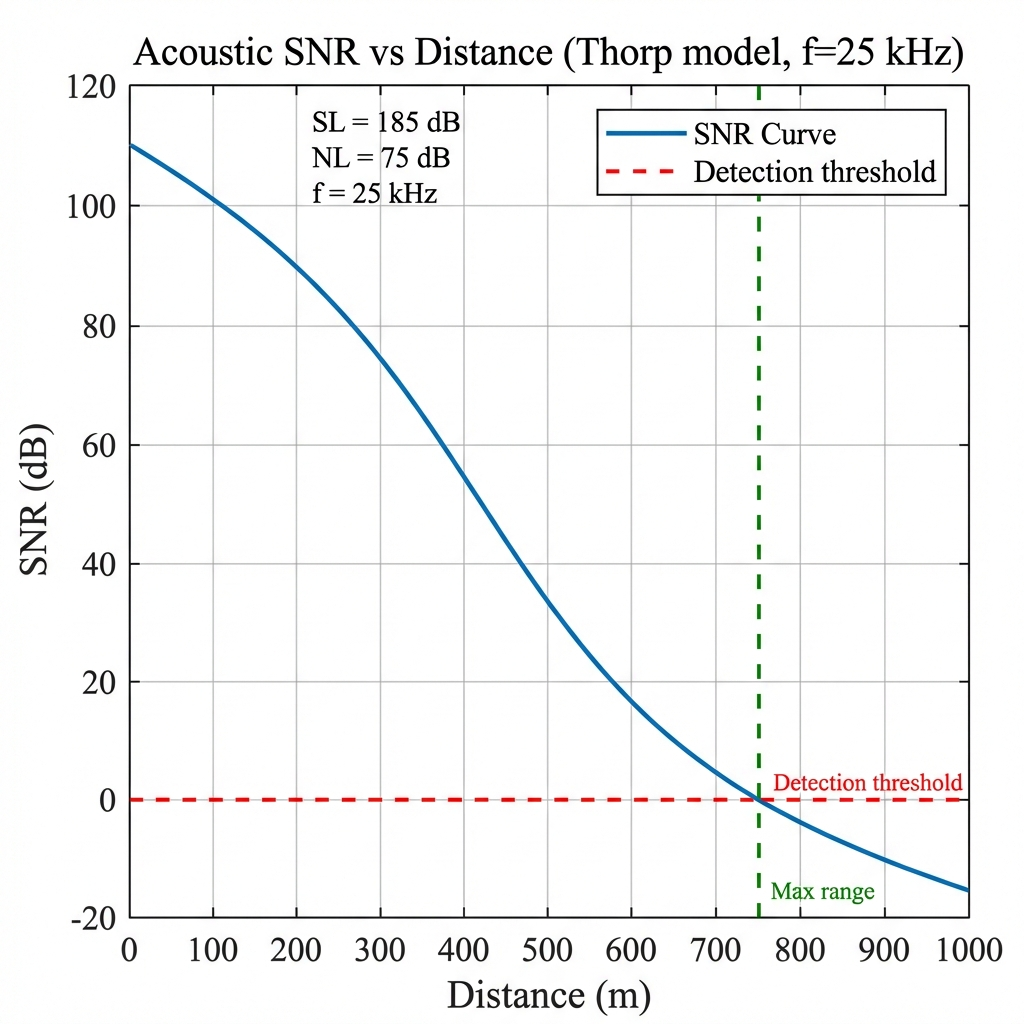
\includegraphics[width=\linewidth]{snr_graph.png}
    \caption{Acoustic SNR computed as a function of distance using Thorp's absorption formula at 25\,kHz.}
    \label{fig:snr}
\end{figure}

% ============================================================================
\section{Conclusions and Future Work}
\label{sec:conclusions}

This work has demonstrated the viability of a lightweight AUV simulator built on ROS\,2 that reproduces the essential operational constraints of the underwater domain. The system successfully integrates a raycasting rendering engine, an acoustic communication channel with a Thorp-based propagation model, a control architecture with subsumption hierarchy for safety, and an onboard autonomy module capable of completing exploration and collection missions.

The iterative development process highlighted the importance of parameter tuning in robotics: the stability of depth control, gripper capture tolerance, and robotic arm speed required multiple empirical adjustment cycles. The documentation of these cycles constitutes a valuable pedagogical contribution, as it illustrates the reality of robotics development beyond theoretical architecture.

\subsection{Identified Limitations}

\begin{itemize}[leftmargin=*,itemsep=2pt]
    \item \textbf{Reactive navigation:} The absence of a global path planner (e.g., Nav2 with A*) limits the AUV's ability to circumnavigate complex obstacles. Straight-line navigation with temporal evasion may result in suboptimal trajectories or deadlocks in adverse geometric configurations.
    \item \textbf{i.i.d.\ packet loss:} The independent loss model does not capture the temporal correlation observed in real acoustic channels. A Markov model (Gilbert-Elliott) would provide greater realism.
    \item \textbf{2D path planning:} Both Nav2 and most ROS\,2 planners are designed for 2D navigation, which limits their direct applicability to an AUV operating in three dimensions.
\end{itemize}

\subsection{Future Work}

\begin{itemize}[leftmargin=*,itemsep=2pt]
    \item Integration of Nav2 for horizontal 2D trajectory planning while retaining the current depth controller.
    \item Correlated acoustic channel model (Gilbert-Elliott) and active application of Doppler shift to control data.
    \item Extension to multi-AUV cooperative scenarios with TDMA acoustic channel access protocols.
    \item Addition of ocean current models affecting both navigation and acoustic propagation.
    \item Integration with \texttt{slam\_toolbox} for simultaneous mapping from the simulated sonar data.
\end{itemize}

% ============================================================================
% REFERENCES
% ============================================================================
\begin{thebibliography}{10}

\bibitem{stojanovic2009}
M. Stojanovic and J. Preisig,
``Underwater Acoustic Communication Channels: Propagation Models and Statistical Characterization,''
\textit{IEEE Commun. Mag.}, vol.~47, no.~1, pp.~84--89, 2009.

\bibitem{uuvsim2016}
M. M. M. Manhaes, S. A. Scherer, M. Voss, L. R. Douat, and T. Rauschenbach,
``UUV Simulator: A Gazebo-based package for underwater intervention and multi-robot simulation,''
\textit{Proc. IEEE OCEANS}, 2016.

\bibitem{stonefish2020}
M. Cie\'{s}lak,
``Stonefish: An Advanced Open-Source Simulation Tool Designed for Marine Robotics, with a ROS Interface,''
\textit{Proc. IEEE OCEANS}, 2019.

\bibitem{thorp1967}
W. H. Thorp,
``Analytic Description of the Low-Frequency Attenuation Coefficient,''
\textit{J. Acoust. Soc. Am.}, vol.~42, no.~1, p.~270, 1967.

\bibitem{urick1983}
R. J. Urick,
\textit{Principles of Underwater Sound}, 3\textsuperscript{rd} ed.
Peninsula Publishing, 1983.

\bibitem{brooks1986}
R. A. Brooks,
``A Robust Layered Control System for a Mobile Robot,''
\textit{IEEE J. Robot. Autom.}, vol.~2, no.~1, pp.~14--23, 1986.

\bibitem{lodev_raycasting}
Lode Vandevenne,
``Raycasting Tutorial,''
\url{https://lodev.org/cgtutor/raycasting.html}, accessed Feb.~2026.

\bibitem{ros2docs}
Open Robotics,
``ROS 2 Documentation: Humble Hawksbill,''
\url{https://docs.ros.org/en/humble/}, 2022.

\bibitem{quigley2009}
M. Quigley \textit{et al.},
``ROS: an open-source Robot Operating System,''
\textit{Proc. ICRA Workshop on Open Source Software}, 2009.

\bibitem{nav2}
S. Macenski \textit{et al.},
``The Marathon 2: A Navigation System,''
\textit{Proc. IEEE/RSJ IROS}, 2020.

\end{thebibliography}

\end{document}
